%%%%%%%%%%%%%%%%%%%%%%%%%%%%%%%%%%%%% 
%% LE2I beamer template
%% Guillaume Lemaitre, October 2014
%%%%%%%%%%%%%%%%%%%%%%%%%%%%%%%%%%%%% 

\documentclass{beamer}

\usepackage[utf8]{inputenc}
\usepackage[T1]{fontenc} 
\usetheme{le2i} 

%% The amssymb package provides various useful mathematical symbols
\usepackage{amssymb}
%% The amsthm package provides extended theorem environments
\usepackage{amsthm}
%% amsmath for math environment
\usepackage{amsmath}

\DeclareMathOperator*{\argmin}{arg\,min}
\DeclareMathOperator*{\argmax}{arg\,max}
\DeclareMathOperator*{\sign}{sign}

%% figure package
\usepackage{epsf,graphicx}
\usepackage{epstopdf}
\usepackage{subfigure}
\usepackage{transparent}

%% In order to draw some graphs
\usepackage{tikz,xifthen}
\usepackage{tikz-qtree}
\usepackage{adjustbox}
\usetikzlibrary{decorations.pathmorphing}
\usetikzlibrary{fit}
\usetikzlibrary{backgrounds}
\usetikzlibrary{shapes,arrows,shadows}
\usetikzlibrary{calc,decorations.pathreplacing,decorations.markings,positioning}
\usetikzlibrary{snakes,decorations.text,shapes,patterns}
% \usepackage{scalefnt,lmodern,booktabs}

%% Package for cross and tick symbols
\usepackage{pifont}
\newcommand{\tick}{\color{green!60!black!80}\ding{51}}
\newcommand{\cross}{\color{red!60!black!80}\ding{55}}

\title{Introduction to Image Processing}
\author{Guillaume Lema\^itre \\ \texttt{guillaume.lemaitre@udg.edu}}
\date{Lecture 1 \\ 16\textsuperscript{th} Sept. 2015}

\institute{Universit\'e de Bourgogne} 

%% Uncomment if you want to avoid thousand of bullet inside the menu
% \usepackage{etoolbox}
% \makeatletter
% \patchcmd{\slideentry}{\advance\beamer@xpos by1\relax}{}{}{}
% \def\beamer@subsectionentry#1#2#3#4#5{\advance\beamer@xpos by1\relax}%
% \makeatother

\begin{document}

% Show the title page
\begin{frame}
  \titlepage
\end{frame}

% Show the table of contents
\begin{frame}
  \tableofcontents[sectionstyle=show,subsectionstyle=show,subsubsectionstyle=hide]
\end{frame}

\section{Human Vision}

\subsection{Human eye}

\begin{frame}
  \frametitle{Human Vision}
  \framesubtitle{Human eye}
  \begin{block}{From the eye to a camera}
    \begin{columns}
      \begin{column}{.5\linewidth}
        \begin{center}
          \only<1>{Choroid}
          \only<2>{Ciliary body \& iris}
          \only<3>{Lens}
          \only<4>{Retina}
          \only<5>{Cones}
          \only<6>{Rods}
          \only<7>{Cones \& Rods}
          \only<8>{Fovea}
        \end{center}
        \begin{itemize}\scriptsize
          \only<1>{\item Composed of blood vessels serving as source of nutrition
          \item Avoid the entrance of external light or backscatter
          \item See relation with physics experiments}
          \only<2>{\item Control the amount of light (2 mm to 8 mm)
          \item Relation with the camera aperture}
          \only<3>{\item Made of fibrous cells and attached to ciliary body
          \item Absorb 8 \% of visible light and all the IR and UV
          \item Cataract diseases
          \item Idem to an optical lens}
          \only<4>{\item Contains 2 types of discrete light receptors: the cones and the rods
          \item Myopia \& hyperopia}
          \only<5>{\item Account for about 6 to 7 million per eye
          \item Are sensitive to color and details
          \item Each one connected to a single nerve end
          \item Cone vision is called \emph{photopic} and is sensitive to high levels of illumination
          \item Similar to a high frequency receptor}
          \only<6>{\item Account for 75 to 150 millions per eye
          \item Not involved in color
          \item Give a general and overall picture of the FOV
          \item Several rods connected to a single nerve end
          \item Sensitive to low levels of illuminations: \emph{scotopic}
          \item Similar to a low frequency receptor}
          \only<7>{\item Symmetrically distributed
          \item Note the presence of the blind spot}
          \only<8>{\item Localisation of the cones in this area
          \item 1.5 mm $\times$ 1.5 mm
          \item 150,000 elts/mm\textsuperscript{2} to 337,000 elts/mm\textsuperscript{2}
          \item CCD imaging ship would need a 5 mm $\times$ 5 mm to achieve similar density}
        \end{itemize}
      \end{column}
      \begin{column}{.5\linewidth}
        \only<1-6>{\begin{figure}
            \centering
            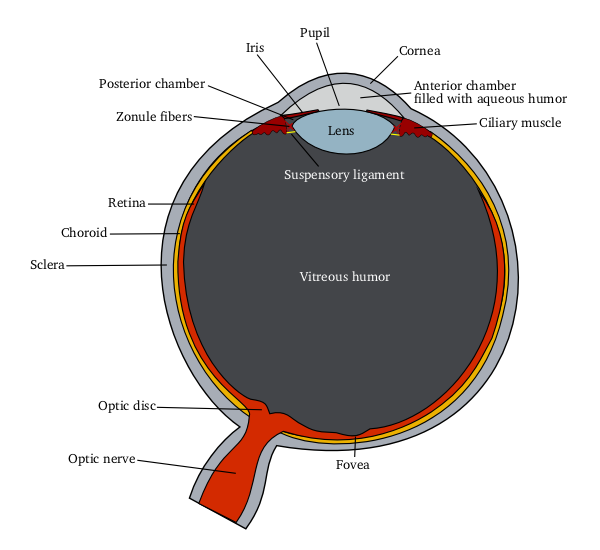
\includegraphics[width=.9\textwidth]{./images/eye.png}
          \end{figure}}
        \only<7>{\begin{figure}
            \centering
            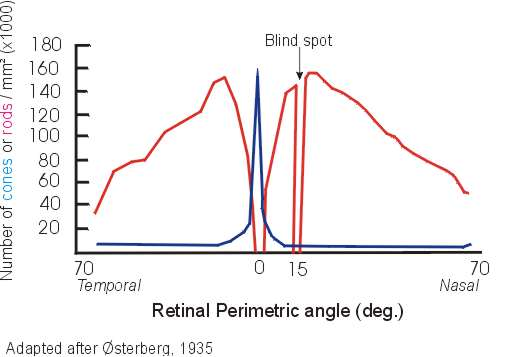
\includegraphics[width=.9\textwidth]{./images/distri.jpg}
          \end{figure}}
        \only<8>{\begin{figure}
            \centering
            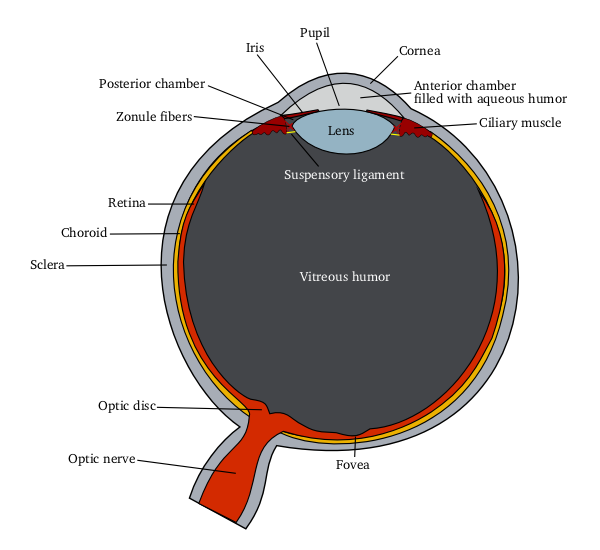
\includegraphics[width=.9\textwidth]{./images/eye.png}
          \end{figure}}
      \end{column}
    \end{columns}    
  \end{block}
\end{frame}

\subsection{Image formation in the eye}

\begin{frame}
  \frametitle{Human Vision}
  \framesubtitle{Image formation in the eye}
  \begin{block}{Example}
    \begin{figure}
      \centering
      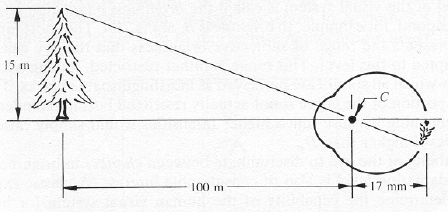
\includegraphics[width=.7\textwidth]{./images/form.png}
    \end{figure}
    \begin{itemize}\scriptsize
    \item Focal length varies from 17 mm to 14 mm
    \item Perception takes place by the relative excitation of light receptors.
    \item The receptors transform this energy to electrical impulses
    \end{itemize}
  \end{block}
\end{frame}

\subsection{Brightness adaptation \& discrimination}

\begin{frame}
  \frametitle{Human Vision}
  \framesubtitle{Brightness adaptation \& discrimination}
  \begin{block}{Human visual system}
    \begin{itemize}\scriptsize
    \item The human vision system (HVS) can adapt to $10^{10}$ light intensity levels
    \item Subjective brightness is a logarithmic function of the light intensity incident on the eye
      \begin{figure}
        \centering
        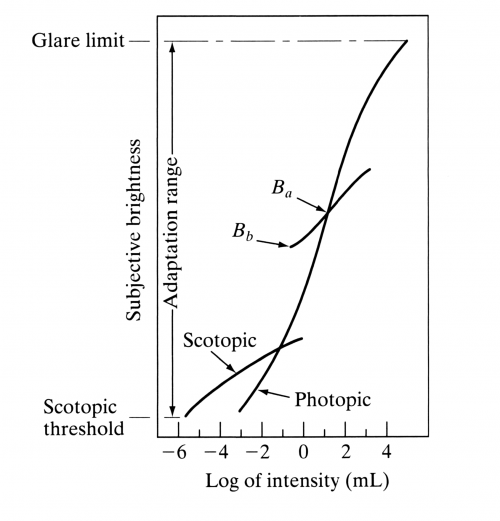
\includegraphics[height=.35\textheight]{./images/sb.png}
      \end{figure}
    \item The HVS cannot operate over such a range simultaneously
    \item For a given set of conditions, the current sensitivity level is called \emph{brightness adaptation level}
    \end{itemize}
  \end{block}
\end{frame}

\begin{frame}
  \frametitle{Human Vision}
  \framesubtitle{Brightness adaptation \& discrimination}
  \begin{block}{Human visual system}
    \begin{itemize}\scriptsize
    \item The eye also discriminates between changes in brightness at any specific adaption level
    \item This is characterised by the Weber ratio
    \end{itemize}
    \begin{equation}
      \frac{\Delta I_c}{I},
    \end{equation}
    {\scriptsize where $\Delta I_c$ is the increment of illumination discriminable 50 \% of the time and $I$ is the background illumination}
  \end{block}
\end{frame}

\begin{frame}
  \frametitle{Human Vision}
  \framesubtitle{Brightness adaptation \& discrimination}
  \begin{block}{Human visual system}
    \begin{figure}
      \centering
      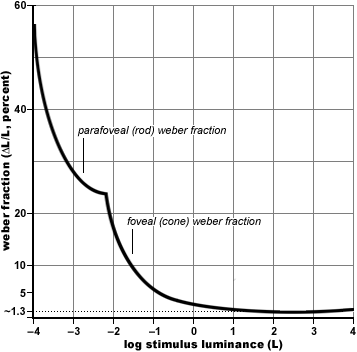
\includegraphics[height=.35\textheight]{./images/wr.png}
    \end{figure}
    \begin{itemize}\scriptsize
    \item Small values of Weber ration mean good brightness discrimination and vice versa
    \item At low levels of illumination brightness discrimination is poor (rods)
    \item It improves significantly as background illumination increases (cones)
    \item The typical observer can discern one to two dozen different intensity changes
    \end{itemize}
  \end{block}
\end{frame}

\begin{frame}
  \frametitle{Human Vision}
  \framesubtitle{Brightness adaptation \& discrimination}
  \begin{block}{Human visual system}
    \begin{itemize}\scriptsize
    \item Overall intensity discrimination is broad due to different set of incremental changes to be detected at each new adaptation level
    \item Perceived brightness is not a simple function of intensity: Mach band effect, simultaneously contrast, and optical effect
    \end{itemize}
  \end{block}
\end{frame}

\begin{frame}
  \frametitle{Human Vision}
  \framesubtitle{Brightness adaptation \& discrimination}
    \only<1>{\begin{block}{Mach band effect}
        \begin{figure}
        \centering
        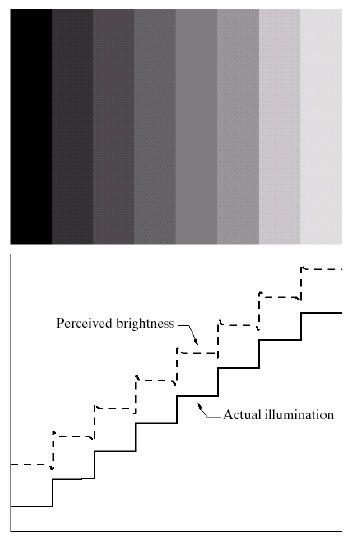
\includegraphics[height=.6\textheight]{./images/mach.png}
      \end{figure}
    \end{block}}
  \only<2>{\begin{block}{Simultaneously contrast}
        \begin{figure}
        \centering
        
\includegraphics[width=.8\textwidth]{./images/sc.png}
      \end{figure}
    \end{block}}
  \only<3>{\begin{block}{Optical effect}
        \begin{figure}
        \centering
        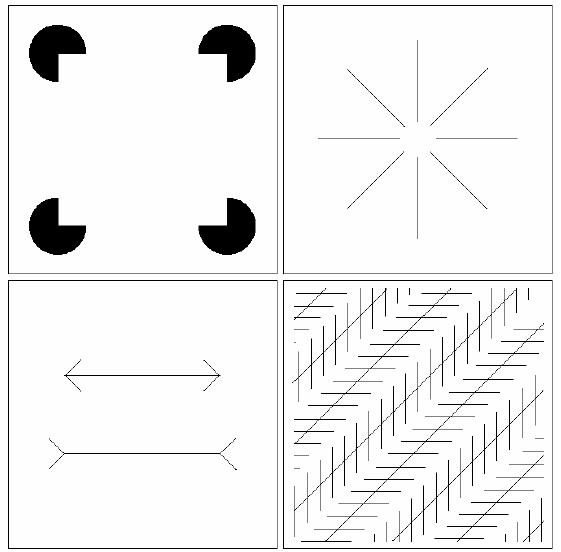
\includegraphics[height=.6\textheight]{./images/oe.png}
      \end{figure}
    \end{block}}
\end{frame}


\end{document}